% !TeX spellcheck = ru_RU
% !TEX root = vkr.tex



%\section{Vivado проект}
%\subsection{Настройки среды}
%\subsection{Состав IP-ядер}
%Готовые блоки:
%\begin{enumerate}
%\item AXI4-Stream Data FIFO,
%\item Utility Vector Logic,
%\item Utility Vector Logic,
%\item FFT,
%\item Complex Multiplier,
%\item Block Memory Generator,
%\item Binary Counter,
%\item Constant,
%\item Simulation Clock Generator,
%\item AXI4-Stream Data Width Converter.
%\end{enumerate}
%
%Собственные блоки:
%\begin{enumerate}
%\item axis\_packet\_demux,
%\item axis\_mux,
%\item fifo\_initializer,
%\item buf\_controller,
%\item fft\_config,
%\item slow\_fifo\_reader,
%\item reference\_reader,
%\item remove\_tail,
%\item packet\_saver.
%\end{enumerate}
%
%Используемые интерфейсы:
%\begin{enumerate}
%\item AXIS.
%\end{enumerate}
%
%Компоненты ПЛИС-обнаружителя:
%\begin{enumerate}
%\item double\_buffering,
%\item last\_samples\_buffer,
%\item FFT,
%\item repeater (один отсчет спектра сигнала повторяется k раз для умножения на k преамбул),
%\item repeater\_delay (задержка в 2 такта для выравнивания спектра сигнала и спектра преамбулы),
%\item Complex Multiplier,
%\item AXI4-Stream Data Width Converter (упаковывает 4 отсчета по 32 бита в одно слово 128 бит для подачи на вход многоканального IFFT),
%\item Обратное FFT,
%\item remove\_tail (в каждом входном пакете обртаного fft валидны лишь некоторое количество первых отсчетов, остальные данные отбрасываются)
%\item packet\_saver (во время симуляции отписывает данные в файл; позже этот файл считывается и обрабатывается python-скриптом с целью анализа и визуализации результатов расчета корреляции).
%\end{enumerate}
%
%\subsection{Настройки IP-ядер}
%Параметры системы указаны в таблицах.
%\begin{table}[h]
%	\centering
%	\begin{tabular}{|p{8cm}|c|}
%		\hline
%		Параметр & Значение \\
%		\hline
%		Тактовая частота АЦП & 10{,}4 МГц \\
%		\hline
%		Коэффициент децимации & 26 \\
%		\hline
%		Частота дискретизации сигнала после децимации & 100 кГц \\
%		\hline
%		Длина преамбулы & 480 отсчётов \\
%		\hline
%		Количество обрабатываемых частотных сдвигов преамбулы & 4 \\
%		\hline
%		Разрядность АЦП & 12 бит \\
%		\hline
%	\end{tabular}
%	\caption{Параметры системы}
%\end{table}
%
%\begin{table}[h]
%	\centering
%	\begin{tabular}{|c|c|c|}
%		\hline
%		Параметр & Прямое FFT & Обратное FFT \\
%		\hline
%		Каналы & 1 & 4 \\
%		\hline
%		Размер преобразования & 2048 & 2048 \\
%		\hline
%		Число тактов преобразования & 15549 & 15549 \\
%		\hline
%		Архитектура & Radix-2, Burst I/O & Radix-2, Burst I/O \\
%		\hline
%		BRAM & 4 & 8 \\
%		\hline
%		DSP & 13 & 20 \\
%		\hline
%	\end{tabular}
%	\caption{Параметры FFT-преобразований}
%\end{table}



\section{Архитектура}

Разработка ПЛИС-обнаружителя выполняется для платформы PLutoSDR+, построенной на базе SoC (ARM + FPGA) и приемопередатчика AD9363.  

В качестве основы используется открытая HDL-прошивка из репозитория\footnote{\url{https://github.com/analogdevicesinc/hdl}} компании Analog Devices.  
Для устройства PLuto SDR+ применяется проект\footnote{\url{https://github.com/analogdevicesinc/hdl/tree/main/projects/pluto}},  
который содержит как аппаратную (HDL), так и программную (C) части системы.

Программный код, исполняемый на процессоре ARM, выполняет:
\begin{itemize}
	\item инициализацию периферии;
	\item конфигурирование AD9363 (по протоколу SPI);
	\item запуск механизма передачи данных через DMA.
\end{itemize}

После настройки приемника оцифрованные отсчёты АЦП поступают в ПЛИС, где далее передаются по внутреннему цифровому тракту и могут быть считаны процессором через DMA с размещением данных в памяти DDR.

\subsection{Место ПЛИС-обнаружителя в системе}

Разрабатываемый ПЛИС-обнаружитель встраивается в существующую HDL-архитектуру после узла формирования комплексных отсчётов АЦП и до блока DMA.  

Таким образом, поток данных в модифицированной системе имеет вид:

\begin{center}
	AD9363 $\rightarrow$ входной интерфейс ПЛИС $\rightarrow$ ПЛИС-обнаружитель $\rightarrow$ DMA $\rightarrow$ DDR
\end{center}

Обнаружитель функционирует полностью внутри логической части (PL) и не требует промежуточной передачи данных в процессорную систему (PS). Это позволяет выполнять корреляционную обработку непосредственно в потоке входных данных без дополнительной нагрузки на интерфейсы PS--PL.

\subsection{Формат входных данных}

Приемопередатчик AD9363 формирует поток комплексных отсчётов сигнала. Каждый отсчёт представлен 24-битным числом комплексного формата:
\begin{itemize}
	\item 12 бит --- действительная компонента (I);
	\item 12 бит --- мнимая компонента (Q).
\end{itemize}

%Во входном интерфейсе ПЛИС выполняется:
%\begin{itemize}
%	\item приём дифференциальных сигналов;
%	\item преобразование их во внутренний логический формат;
%	\item сборка последовательных фрагментов данных в 24-битные комплексные отсчёты.
%\end{itemize}

На выходе данного узла формируется синхронный поток комплексных отсчётов I/Q фиксированной разрядности, тактируемый сигналом, производным от тактовой частоты АЦП. Именно этот поток подаётся на вход ПЛИС-обнаружителя.

\subsection{Назначение и интерфейсы обнаружителя}

Разрабатываемый ПЛИС-обнаружитель предназначен для вычисления взаимнокорреляционной функции входного комплексного сигнала с эталонной преамбулой при заданном наборе частотных гипотез. На вход модуля поступает поток комплексных отсчётов, сформированных после цифровой обработки в приёмном тракте.

Результатом функционирования обнаружителя является поток отсчётов корреляционной функции, формируемый для каждого рассматриваемого частотного сдвига. Данный поток передаётся в существующий тракт прямого доступа к памяти (DMA) и далее записывается в оперативную память системы.

Включение обнаружителя в цифровой тракт приводит к изменению состава передаваемых данных между логической частью (PL) и процессорной системой (PS): вместо исходных отсчётов АЦП в память передаются результаты корреляционной обработки. При этом механизм конфигурирования приёмного тракта и структура интерфейса DMA сохраняются без изменений.








\section{Архитектура ПЛИС-обнаружителя}

\subsection{Общая организация вычислительного тракта}

Архитектура обнаружителя разработана в среде Vivado с использованием инструмента проектирования \textit{IP Integrator}, предназначенного для построения системы из готовых IP-ядер и пользовательских модулей с графическим описанием их взаимосвязей.

\begin{figure}[h]
	\centering
	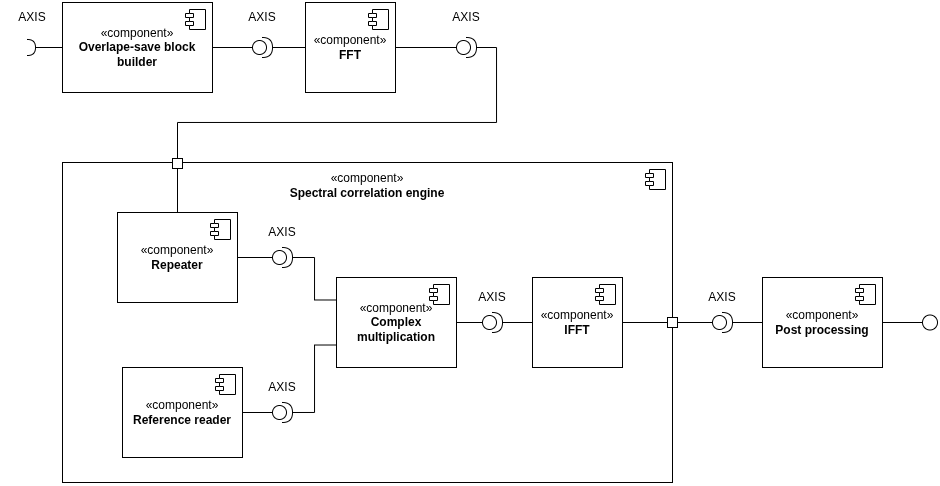
\includegraphics[
	width=\textwidth
	]{pics/fpga-finder-march-7-2025.drawio.png}
	\caption{Диграмма компонентов ПЛИС-обнаружителя.}
	\label{fig:correlation_all}
\end{figure}

В основе решения лежит потоковый принцип обработки данных с применением интерфейса AXI4-Stream (AXIS). Передача информации между функциональными блоками осуществляется в виде последовательности отсчётов, объединённых в пакеты фиксированной длины. Обмен сопровождается стандартными служебными сигналами интерфейса AXIS, в том числе сигналом наличия корректных данных (\texttt{tvalid}) и сигналом завершения пакета (\texttt{tlast}). Такой подход обеспечивает упорядоченную и синхронизированную передачу данных между модулями без использования общей адресной памяти.

Назначение разработанной архитектуры --- вычисление взаимной корреляции входного сигнала с преамбулой длиной 480 отсчётов для четырёх различных частотных гипотез. Корреляция вычисляется непрерывно без разрывов между соседними блоками обработки.

Входной поток формируется после децимации сигнала с коэффициентом 26. При тактовой частоте АЦП 10,4 МГц частота дискретизации после децимации составляет 100 кГц. Далее поток комплексных отсчётов поступает в тракт корреляционной обработки.

В работе обнаружителя можно выделить следующие этапы:

\begin{enumerate}
	\item формирование блока данных для БПФ с учётом перекрытия;
	\item прямое БПФ входного сигнала;
	\item умножение спектра сигнала на спектры частотно-смещённых преамбул;
	\item многоканальное обратное БПФ;
	\item удаление некорректной части результата;
	\item передача результатов на выходной поток.
\end{enumerate}

%Движение данных через систему организовано таким образом, что каждый новый блок входных отсчётов частично перекрывается с предыдущим, обеспечивая реализацию линейной корреляции методом быстрой свёртки.

\subsection{Корреляция через БПФ}

Взаимная корреляция дискретных комплексных сигналов определяется выражением

\begin{equation}
	R_{xy}[n] = \sum_{m=0}^{K-1} x[m+n]\, y^*[m],
\end{equation}

где $K = 480$ --- длина преамбулы, а $y^*$ обозначает комплексное сопряжение.

Корреляция эквивалентна свёртке сигнала $x[n]$ с временно инвертированным и сопряжённым сигналом $y[n]$:

\begin{equation}
	R_{xy}[n] = x[n] * h[n], \qquad h[n] = y^*[-n].
\end{equation}

Согласно теореме о свёртке \cite{oppenheim_dsp}:

\begin{equation}
	\mathcal{F}\{x[n] * h[n]\} = X[k] \cdot H[k],
\end{equation}

где $\mathcal{F}$ --- дискретное преобразование Фурье.  

Следовательно, корреляцию можно вычислять в частотной области:

\begin{equation}
	R_{xy}[n] = \mathcal{F}^{-1}\{X[k] \cdot H[k]\}.
\end{equation}

При длине блока $N = 2048$ вычислительная сложность прямого расчёта корреляции порядка $O(NK)$ становится существенно выше, чем сложность алгоритма БПФ $O(N \log N)$. Поэтому в архитектуре применяется метод быстрой корреляции через прямое и обратное БПФ.

\subsection{Переход от циклической свёртки к линейной}

Преобразование Фурье реализует циклическую свёртку. Для получения линейной корреляции используется блочный метод с перекрытием --- схема overlap-save, подробно описанная в \cite{oppenheim_dsp}, \cite{smith_dspguide}.

Пусть:
\begin{itemize}
	\item $N = 2048$ --- длина БПФ;
	\item $K = 480$ --- длина преамбулы;
	\item $L = N - K + 1 = 1569$ --- число корректных отсчётов на блок.
\end{itemize}

Каждый входной блок формируется следующим образом:
\begin{itemize}
	\item первые $K-1 = 479$ отсчётов --- последние отсчёты предыдущего блока;
	\item оставшиеся $L$ отсчётов --- новые данные входного потока.
\end{itemize}

После выполнения обратного БПФ первые $K-1$ отсчётов результата отбрасываются как искажённые циклической свёрткой. Оставшиеся $L$ отсчётов являются корректным фрагментом линейной корреляции.

В архитектуре это реализуется аппаратно следующим образом:

\begin{itemize}
	\item модуль \textbf{last\_samples\_buffer} хранит 479 последних отсчётов предыдущего блока;
	\item модуль \textbf{double\_buffering} обеспечивает непрерывную подачу 2048 отсчётов на вход БПФ;
	\item модуль \textbf{remove\_tail} отбрасывает первые 479 отсчётов результата обратного БПФ.
\end{itemize}

Таким образом, поток данных организован как последовательность перекрывающихся блоков длиной 2048 отсчётов, что гарантирует отсутствие разрывов и артефактных значений корреляционной функции на границах блоков данных.

\subsection{Формирование и хранение спектров преамбул}

Для компенсации возможного частотного рассогласования предусмотрена обработка четырёх частотных гипотез. Каждая гипотеза соответствует частотному сдвигу $\Delta f_i$ во временной области:

\begin{equation}
	s_i[n] = s[n] e^{j2\pi \Delta f_i n T_s}.
\end{equation}

Спектры всех четырёх вариантов преамбулы:
\begin{itemize}
	\item предварительно вычисляются вне ПЛИС;
	\item комплексно сопрягаются;
	\item сохраняются в блочной памяти (Block Memory Generator).
\end{itemize}

Во время работы системы модуль \textbf{reference\_reader} синхронно считывает спектральные коэффициенты из BRAM и подаёт их на вход комплексных умножителей.

\subsection{Обработка спектра входного сигнала}

После формирования блока длиной 2048 отсчётов данные поступают в ядро FFT (Radix-2, Burst I/O). Выходной спектр представляет собой поток комплексных значений, передаваемых через интерфейс AXIS.

Для обеспечения параллельной обработки четырёх частотных гипотез каждый спектральный отсчёт входного сигнала дублируется модулем \textbf{repeater}. Таким образом формируется четыре параллельных потока данных, которые далее перемножаются с соответствующими спектрами преамбул в блоке Complex Multiplier.

Поскольку ядро обратного БПФ сконфигурировано как четырёхканальное, далее выполняется упаковка четырёх 32-битных комплексных отсчётов в одно 128-битное слово с помощью AXI4-Stream Data Width Converter. Это позволяет синхронно выполнить четыре независимых IFFT в одном IP-ядре.

\subsection{Обратное БПФ и формирование выходного потока}

Многоканальное IFFT (размер 2048) формирует четыре временных последовательности корреляции.  

Каждый входной пакет длиной 2048 отсчётов преобразуется в 2048 отсчётов результата, из которых 479 являются некорректными согласно методу overlap-save. Модуль \textbf{remove\_tail} удаляет эту часть, после чего оставшиеся 1569 отсчётов передаются в выходной поток.

Передача организована пакетами AXIS с корректным формированием сигнала TLAST, что обеспечивает согласованность с последующими блоками обработки или средствами моделирования.

\subsection{Организация управления потоками}

Поскольку ядра FFT используют режим Burst I/O, обработка выполняется блоками фиксированной длины. Для исключения пауз между блоками применена схема двойной буферизации. Пока один буфер передаётся в FFT, второй заполняется новыми входными данными.

Модули:
\begin{itemize}
	\item \textbf{axis\_packet\_demux},
	\item \textbf{axis\_mux},
	\item \textbf{buf\_controller},
	\item \textbf{slow\_fifo\_reader}
\end{itemize}
обеспечивают согласование скоростей потоков, управление пакетами и корректное формирование управляющих сигналов AXIS.

Таким образом, движение данных в системе описывается следующей схемой:

\begin{center}
	входной поток $\rightarrow$ формирование блока $\rightarrow$ FFT $\rightarrow$ спектральное умножение $\rightarrow$ IFFT $\rightarrow$ удаление хвоста $\rightarrow$ выходной поток.
\end{center}





